\chapter{Building Accessible and Automated Mass Cytometry Analysis Tools}
\label{03cygnal}

\section{Introduction}


As outlined in the background section, the mass cytometry platform used to analyse the CRC organoids is already a mature approach. With a previously characterised model, the effects of both TME and genotypical perturbations have also been described, but the data analysis was done using custom and discrete scripts; encumbering consistency and reproducibility for future analyses. Manual gating too for cell state.

% cygnasl
To improve upon this I have designed and developed CyGNAL (CyTOF SiGNalling AnaLysis)20, a pipeline for mass cytometry data analysis with a focus on studying PTM changes across multiple conditions. 
\colorbox{yellow}{Under continued development and in revision at Nature Protocols, CyGNAL aims to streamline and bring to non-computational scientists analyses similar to those shown in Qin et al. 202011, with the addition of dimensionality reduction embeddings and interactive visualisations.}
Applied to analsie datasets, works in conjucntion with tobis mc and multiplexed cytof panels on organoids as shown in Sufi \& Qin et al. \cite{sufi_multiplexed_2021}.

%class
The maturity of the platform is also reflected on the properties of the markers used in the mass cytometry panels, with the most robust markers achieving highly binary and specific staining. Given the importance of cell state changes to perturbations in the epithelial organoids, either in the form of intrinsic effects such as genotype or extrinsic in the form of the TME or drug treatments, an automated approach of labelling and assigning a cell state to each cell in an experiment would facilitate routine analysis of mass cytometry datasets. 
I thus hypothesise that we can use a machine learning approach to, using a series of canonical cell state markers, automatically predict and label the hundreds of thousands of cells captured in a mass cytometry experiment. To this end I aim to develop a random-forest classifier. This classifier will be able to ingest mass cytometry datasets and, using manually gated datasets with cell state labels as training data, label each of the cells with one of six possible cell states: Apoptosis, G0, G1, S-phase, G2, and M-phase. 

\section{CyGNAL: CyTOF Signalling Analysis pipeline}

\subsection{Workflow}
% \subsection{}{Pipeline modules}

Previous to analysing the data in CyGNAL, mass cytometry datasets are debarcoded as needed (using the tool in https://github.com/zunderlab/single-cell-debarcoder) and initial data pre-processing and quality control is carried in Cytobank (https://www.cytobank.org/) (see the leftmost section of Figure 1). In that platform, the single cells are gated for Gaussian parameters, their DNA content, and uptake of cisplatin using manual gates. Gating on cell state and cell type specific markers can also be done in order to both eliminate doublets but also to identify cells belonging to each state or type; information which can then be used to train the cell state classifier among others.

Installation. Distribution as a container hosted in dockerhub. can also be used by downloading the project (hosted in github) and then installing all required Python and R dependencies via conda using the YML environment file.


\colorbox{yellow}{ADD USER INPUTS AND DIRECTIONS TO EACH OF THE STEPS}

In brief, the preprocessing step formats and exports the heavy metal channels (based on the naming convention of the Fluidigm CyTOF software), embeds the metadata of the experiment and assigns each event within the dataset a unique cell index. 


Dimensionality reduction (e.g., uniform manifold approximation and projection (UMAP)50) can be performed on cell-comprised datasets and is mainly used as a visualization tool in our workflow (Fig. 6c). Cells can be assigned a cell-type identity via biaxial gating (Fig. 6d), followed by cell-state identification and PTM analysis in a cell type–specific manner (Fig. 6e,f). 


Earth mover’s distance (EMD)51,52 is used to quantify PTM node intensity, and density resampled estimation of mutual information (DREMI)53 is used to score PTM-PTM edge connectivity. 


Multiple EMD/DREMI values can be visualized with heatmaps and further summarized by using principal component analysis (PCA). When paired with a well-curated antibody panel and robust experimental design, TOBis MC allows multiplexed analysis of cell type–specific PTM signaling of heterocellular organoids17.


FUrthermore, utils folder has optional steps that either complement the main ones or belong to additional utilities for handling mass cytometry datasets. Feedbakc from users int he lab paramount when defining these utilities.

\begin{figure}
    \centering
    \includegraphics{03cygnal/figs/3CyGNALpipeline.png}
    \caption{cell types and stem niches and regulation}
    \label{fig:fig2}
\end{figure}

Step-by-step instructions and troubleshooting steps found in Sufi \& Qin et al. 2021 

% \subsubsection{Computational steps}

% \subsubsection{Interactive visualisations}

\subsection{Usage example Results}

Sample data from XXXX. Gated and annotated on cell types and states. \cite{sufi_multiplexed_2021}.

% \subsection{}{Usage example}

% \subsubsection{Figure on using CyGNAL with a cytof organoid dataset}

\begin{figure}
    \centering
    \includegraphics{03cygnal/figs/3CYGNAL_usage.png}
    \caption{}
    \label{}
\end{figure}

Preprocess

Cellular embeddings.
Umap of sample data. Phate of sample data too.

PTM signalling network analysis: EMD and DREMI
Vis with heatmaps. Resulting score can also be used to annotated a PTM signalling diagram (nodes emd score, edge dremi scores) as in \cite{qin_cell-type-specific_2020}.
Heatmaps of 

Cross-condition comparison using PCA. 
Show results. Applied also to EMD data from scrnaseq expression (and not just cytof data), as shown in \cite{cardoso_rodriguez_single-cell_2023}.


\section{Cell-state Random Forest Classifier}

General idea of gating done on limited subset of markers is what determines cell state. Process naturally resembles decision trees (threshold of antody intensity results in binary output). Random forest as an ensemble approach that can automate the gating process.

\begin{figure}
    \centering
    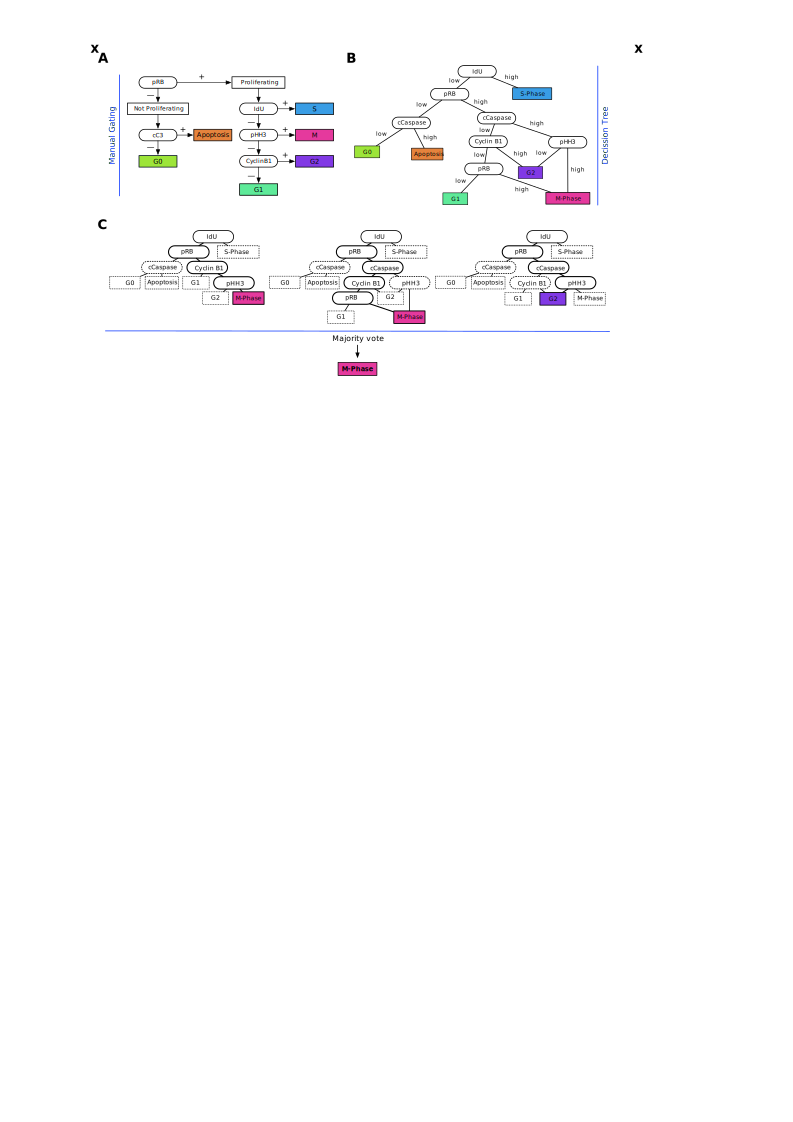
\includegraphics{03cygnal/figs/3CLASS_stateRF.png}
    \caption{}
    \label{}
\end{figure}

\subsection{5-marker model:baseline}

Testing the 5-marker RF model on a single time-point SI LGR5 organoid culture11 results in global accuracy for all classes of 0.93. However, looking at the classification report in Figure 3 a) we see how there is a significant drop of f1-scores when classifying the apoptotic class, scores which otherwise remain above 0.92. This fall in f1-scores seems to be driven by a low precision (0.5) when classifying cells as apoptotic.
Performance of the classifier drops when testing against the CRC TME colonic organoid cultures from Qin et al. 2020. In this case, when we subset just the organoid cells from the organoid cultures (i.e., by extracting all epithelial cells irrespective of the genotype or the other cell types they might have been analysed with), we observe a global accuracy of 0.91. Looking at the classification details (Figure 3 b.) we see a very similar pattern to the SI LGR5 results; with the apoptotic class presenting the lowest f1-scores (0.6) characterised by a low precision (0.43). Furthermore, the remaining f1-scores are also lower overall, with only the S-phase and M-phase classes reaching above the 0.9 mark.
When instead of subsetting just the organoid cells we test against all cells from the CRC TME dataset (i.e., including also fibroblasts and macrophages) global accuracy drops down to 0.87. The relatively high global accuracy does not reflect the failure of the classifier to, yet again, identify the apoptotic cells (see Figure 3 c.). In Figure 3 d) the classification matrix is used to build a dot plot in which the true labels (“Real state” from gating) are compared against the predicted labels (“Predicted state”), highlighting how a majority of the cells labelled as apoptotic are actually G0 cells, explaining the precision of 0.32 for the former class. There is also some confusion around the G2 cells, as a significant number of these cells are classified as either G0 or G1.
 
Figure 3: Benchmarking 5-marker RF cell state classifier. Shown in a), b), and c) are the classification reports obtained from running the 5-marker RF classifier against data manually labelled for cell state (representing the “real state” or ground truth). In a) a single timepoint SI LGR5 dataset was used, very similar to the training data for the model. The dataset in both b) and c) is a coculture of CRC organoids and their TME, with the cells in b) being a subset of the whole dataset containing just epithelial cells. Decreasing levels of performance correlate with increasing differences between the train and test datasets, as can be seen by the low f1-scores for the apoptotic class in c). Using the same data as c), the dot plot derived from the classification matrix in d) depicts the number and proportion (as both size and colour of the circles) of mislabelled cells for each cell state, showing that a considerable number of falsely mislabelled apoptotic cells are actually in G0 phase and some cells. RF: Random Forest.



\subsection{10-marker model improves apoptotic classification}

Cross species, on PDO chemotherapy data.

Preliminary benchmark results from the updated 10-marker implementation using PDO data show improved performance when compared to the 5-marker model. In this case we observe a global accuracy greater than 0.99, with the lowest f1-score being of 0.95 for the cells in M-phase (see Figure 4 a.). In the classification matrix in Figure 4 b) we observe how, given the lower total count of M-phase cells (true label = 5, one order of magnitude smaller than the other classes), small numbers of misclassified cells (mainly as G2 and S-phase predicted labels, represented by the numbers 4 and 3 respectively) drive down the recall for the M-phase class. 
In contrast with the 5-marker model results, there is an apparent lack of issues when classifying the apoptotic class, with only 0.35% of true apoptotic cells being mislabelled. A bar plot representing the importance of each feature during classification is shown in Sup. Figure 2.
 
Figure 4: Benchmarking the new 10-marker RF cell state classifier. Building a RF classifier with an increased number of markers using data from PDOs renders better results than the original 5-marker model, as can be seen in a) with the classification report. b) Classification matrix generated automatically during model building, showing extremely low levels of misclassified cells. RF: Random Forest. PDO: Patient-Derived Organoids. Labels: 0=Apoptosis, 1=G0, 2=G1, 3=S-phase, 4=G2, 5=M-phase.

\subsection{Tested on externally cytof data}



\section{Conclusions}

cygnal can be used for explor analysis and even publi grade results -> do we have ref to substantiate this statement though?

classifier simple model that works due to limited number of markers and gating nature of current manual state classes. Robust and generalisable expected weak points.